\documentclass[11pt]{article}
\usepackage[utf8]{inputenc}
\usepackage[T1]{fontenc}
\usepackage{amsmath}
\usepackage{amsfonts}
\usepackage{amssymb}
\usepackage[version=4]{mhchem}
\usepackage{stmaryrd}
\usepackage{graphicx}
\usepackage[export]{adjustbox}
\graphicspath{ {./images/} }

\begin{document}
\section*{Reading}
Interpreting Standard Deviation and Variance

Perhaps the most important single risk measure in investments is the standard deviation of returns, or volatility. Unfortunately, the complexity of its formula and its computation can lead to a belief that standard deviation is not easily interpreted. But the standard deviation of returns is almost as easy to interpret as the mean (expected value) of the returns. The purpose of the next two sections is to demonstrate the ease with which the standard deviation of returns can be intuitively understood.

\section*{Standard Deviation and Typical Deviations}
The standard deviation of an investment's returns can be very roughly approximated as the typical amount by which an investment's actual return deviates from its average. Standard deviation, or volatility, is such a central concept in investments that we present an example here to encourage an intuitive grasp.

Let's start with applying the concept of standard deviation to basketball scores. Observers of basketball might estimate that an average number of points for one team to score in one game might be 100 and that a typical amount by which the outcomes tend to differ from this expectation might be 15 points. In other words, among the higher-than-average scores, a typical score would be 115 points, while among the lower-than-average scores, a typical score would be 85 points. In this case, 15 points would be a rough estimate of the standard deviation of the basketball score for one team.

The idea is that standard deviation (volatility) is a measure of dispersion that can be roughly viewed on an intuitive basis. In statistics, the average distance between a variable and its mean is known as the mean absolute deviation, but it is usually not very different from the standard deviation. The exact relationship between the standard deviation and the mean absolute deviation depends on the underlying distribution. In the case of the normal probability distribution, the standard deviation is approximately 1.25 times the mean absolute deviation, which probably somewhat understates the magnitude of the difference observed in distributions of most returns from modern financial markets with high kurtosis. However, in most cases of investment returns without extreme events, the concepts of standard deviation and mean absolute deviation are close enough that viewing them as being similar in magnitude facilitates a reasonably clear understanding.

Let's take a look at a portfolio that has an annual expected return of $5 \%$ and a standard deviation of $2 \%$. We should be able to develop a quick and easy intuitive feel for the range of outcomes. In a year of average performance, this portfolio will earn $5 \%$. However, among those years with below-average performance, a typically bad year would generate a $2 \%$ lower return, or about $3 \%$. Sometimes the portfolio would do worse than a $3 \%$ return in a bad year and sometimes perhaps a little better. Of those years with above-average performance, a typically good year would generate a return of perhaps $7 \%$.

If the standard deviation of the asset's return fell to $1 \%$, then we would understand that the returns were clustered closer to $5 \%$, with typically good years producing a return of about $6 \%$ and typically bad years producing a return of around 4\%, each found by either adding or subtracting 1 standard deviation to or from the expected return. Of course, returns could be much higher or much lower, indicating highly unusual circumstances in which the outcomes are many standard deviations from the average.

Once we are familiar with the concept of standard deviation, we can use its mathematical properties to clarify the behavior of risk in a portfolio context and to sharpen our intuition. With a little practice, standard deviation becomes as easy to use as averages.

\section*{Standard Deviation of Normally Distributed Returns}
If the return distribution were exactly normal, we could develop more precise indications of the range of values and their associated probabilities.

The next exhibit depicts the use of standard deviation to specify confidence intervals for normally distributed variables. The diagram at the top of the next exhibit illustrates the range of outcomes that could be expected within 1, 2, or 3 standard deviations from the mean of the distribution. The table at the bottom of the next exhibit indicates the probabilities that a normally distributed variable will lie inside a range of 1,2, or 3 standard deviations (two tails) from the mean, or outside the range in a prespecified direction (single tail).

Confidence Intervals for the Normal Distribution Using Standard Deviation

\begin{center}
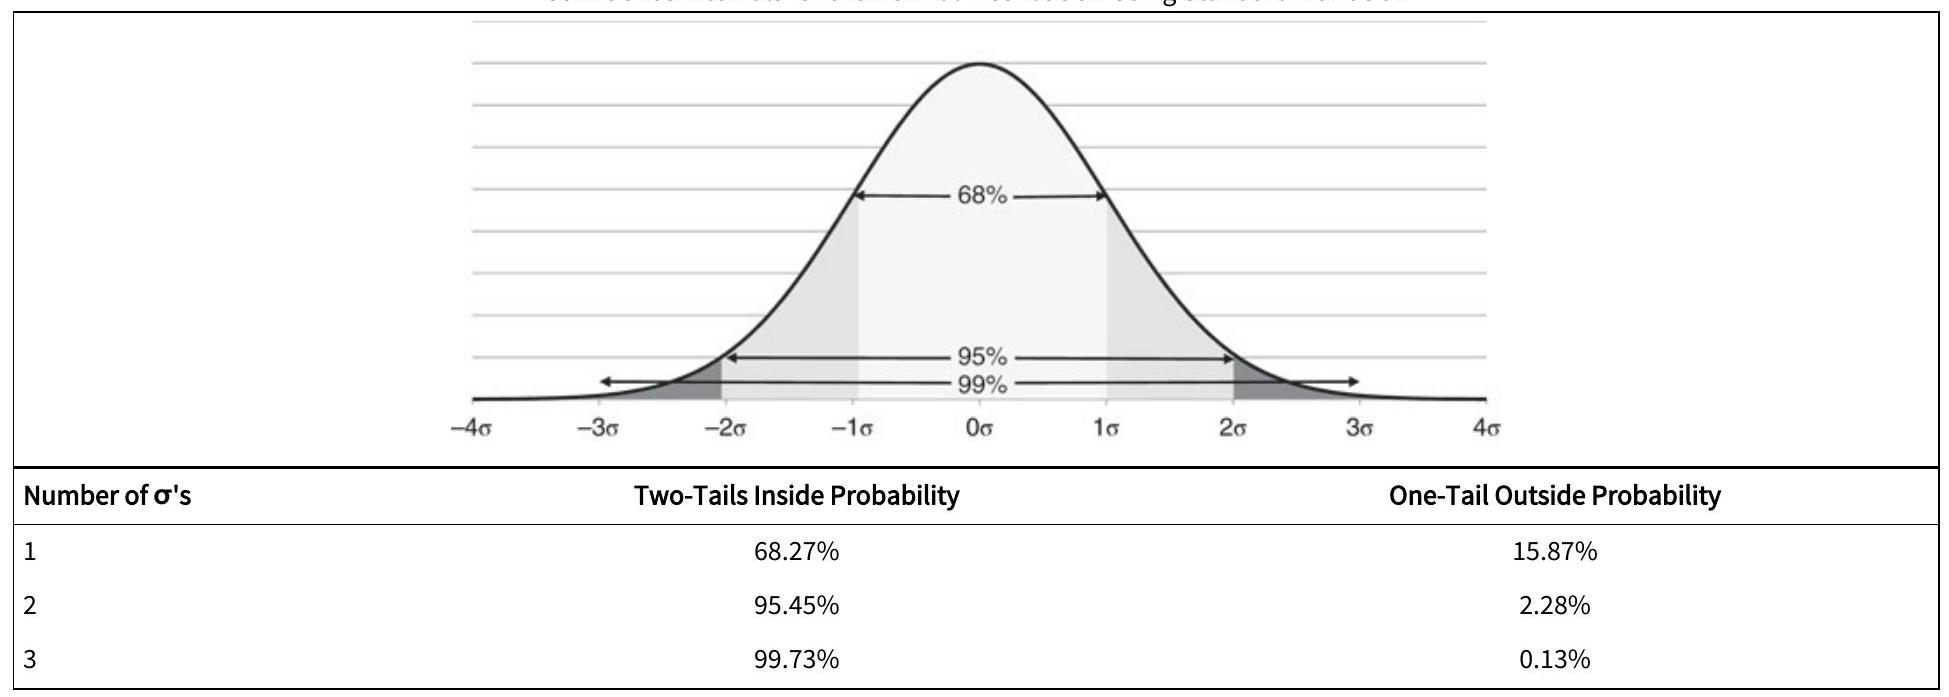
\includegraphics[max width=\textwidth]{2024_04_10_e31febb808c589fc558dg-2}
\end{center}

If returns were normally distributed, the standard deviation of the returns would help an investor know with precision what the probabilities of every outcome would be relative to its mean. Very roughly, two-thirds of the time the returns should lie within 1 standard deviation of the mean. The diagram illustrates this case of a $+/-1$ standard deviation range using the lightest shading on each side of the mean, and illustrates larger ranges using darker shading. The diagram does not illustrate a\\
particular value for the mean and standard deviation. The horizontal axis may be labeled to reflect the value of the mean and standard deviation. In the top panel of above exhibit the value of the mean would lie on the horizontal axis at the point labeled $0 \sigma$. For all other points on the horizontal axis, the value is found by multiplying the standard deviation by the indicated number of standard deviations and adding the value to the mean. For example, with a mean return of $5 \%$ and a standard deviation of $2 \%$, two-thirds of the outcomes (more exactly, $68.27 \%$ ) would tend to lie between $3 \%$ and $7 \%$ (found as $-2 \%$ and $+2 \%$ from the mean of $+5 \%$ ). Also, roughly $95 \%$ of the time, the returns should lie within 2 standard deviations (between $1 \%$ and $9 \%$ ). The one-tail probabilities would inform an investor that in this same example, there would be about a $16 \%$ probability that the return would be less than $3 \%$, and a $2.28 \%$ probability that the return would be less than $1 \%$. The normal distribution is symmetric, so there would be a $0.13 \%$ probability that the return would be more than $11 \%$.

As discussed previously, actual return distributions are usually non-normally distributed. However, the large differences between the normal distribution and the actual distributions of returns typically observed in financial markets tend to occur farther out into the tails, such as 4 or more standard deviations. So for many actual return distributions, the probabilities just given would serve as reasonable approximations.

However, for huge return aberrations, such as a move of 10 standard deviations, the normal distribution provides an astoundingly underestimated indication of the actual probabilities of tail events. Extreme tail events, such as the U.S. equity market's decline during the fourth quarter of 2008, can be hundreds or even thousands of times more likely than indicated by probabilities from the normal distribution and historical standard deviations.

Standard deviation is analyzed so often in the context of the normal distribution that it is sometimes easy to forget that statements such as "Roughly $95 \%$ of the outcomes lie within 2 standard deviations of a mean" implicitly assume that the distribution is normally or near-normally distributed. Care should be taken to understand the assumed underlying probability distribution before associating outcomes with probabilities.

\section*{Properties of Variance}
There are useful properties of variance in the analysis of alternative investments. Variance works well in many formulas regarding risk. This section demonstrates an important property of the variance of the returns of an asset through time. The variance of an investment's return over a time interval of $T$ periods can be expressed as $T$ times the variance measured over a single period under particular assumptions.

\section*{FOUNDATION CHECK}
The material in the Properties of Variance section assumes familiarity with mean and variance as applied within a Markowitz framework.

We begin with the well-known formula for the variance of the return of a portfolio ( $p$ ) of $n$ assets as a weighted average of the variances and covariances of the returns of the assets in the portfolio:


\begin{equation*}
\sigma_{p}^{2}=\sum_{i=1}^{n} \sum_{j=1}^{n} w_{i} w_{j} \operatorname{Cov}\left(R_{i}, R_{j}\right) \tag{1}
\end{equation*}


where $w_{i}$ and $w_{j}$ are the weights of assets $i$ and $j$ in the portfolio.

Note that the covariance of any variable with itself is equal to its variance. Thus, Equation 1 contains $n$ variances (one for each of the $n$ assets) and $n^{2}-n$ covariances (from the pairs of assets). The additivity of the formula assists in financial modeling, such as Markowitz's pioneering work on risk and return, in which variance measured risk. In the case of uncorrelated returns between securities, this formula is simplified because all of the covariances between nonidentical assets are zero:


\begin{equation*}
V\left(R_{p}\right)=\sum_{i=1}^{n} w_{i}^{2} \operatorname{Var}\left[R_{i}\right] \quad \text { when } \rho=0 \text { between all individual assets } \tag{2}
\end{equation*}


where $R_{p}$ is the portfolio's return, and $\rho$ is the correlation coefficient between all individual assets.

An important analogous concept involves the computation of the variance of a multiperiod return. The multiperiod continuously compounded rate of return of any asset is the sum of the continuously compounded returns corresponding to the sub-periods, as noted earlier in the session Quantitative Foundations. For instance, the weekly rate of return expressed as log return is the sum of the five daily log returns:


\begin{equation*}
R_{w}^{m=\infty}=R_{1}^{m=\infty}+R_{2}^{m=\infty}+\cdots+R_{5}^{m=\infty} \tag{3}
\end{equation*}


where $R_{w}^{m=\infty}$ represents the weekly log return.

If we assume that the returns are uncorrelated through time (i.e., there is no autocorrelation), all covariances vanish, and the variance of the weekly return is the sum of the variances of the daily returns:


\begin{equation*}
V\left(R_{w}\right)=V\left(R_{1}\right)+V\left(R_{2}\right)+V\left(R_{3}\right)+V\left(R_{4}\right)+V\left(R_{5}\right) \text { when } \rho_{t, t-k}=0 \tag{4}
\end{equation*}


If we make the further assumption that the variances of the periodic returns of an asset are constant (i.e., homoskedastic), then the variance of the returns for a $T$ period time interval can be expressed as:


\begin{equation*}
V\left(R_{T}\right)=T \times V\left(R_{1}\right) \text { when } \rho_{t, t-k}=0 \tag{5}
\end{equation*}


Since uncorrelated returns through time are consistent with market efficiency, this equation can be viewed as a starting point for understanding variance across different time horizons for asset returns that are reasonably independent through time. If returns are positively correlated in time (i.e., trending, or positively\\
autocorrelated), then the variance will be larger than specified in Equation 5. If returns are negatively correlated in time (i.e., mean-reverting, or negatively autocorrelated), then the variance will be smaller than specified in Equation 5.

\section*{Properties of Standard Deviation}
The standard deviation has several especially useful properties in the study of the returns of alternative investments. One important property involves perfectly correlated cross-sectional returns. The standard deviation of a portfolio of perfectly correlated assets is a weighted average of the standard deviations of the assets in the portfolio:


\begin{equation*}
\sigma p=\sum_{i=1}^{n} w_{i} \times \sigma_{i} \quad \text { when } \rho_{i j}=1 \text { for all } i, j \tag{6}
\end{equation*}


Another important property of the standard deviation involves a situation in which a return or any random variable can be expressed as a linear combination of another variable:

$$
Y_{t}=m X_{t}+b
$$

where $Y_{t}$ is a random variable, such as the return of asset $Y$ in time $t, X_{t}$ is another random variable, such as the return of asset $X$ at time $t, m$ is a fixed slope coefficient; and $b$ is a constant intercept. The standard deviation of $Y$ is found as the product of the standard deviation of $X$ and the slope coefficient:


\begin{equation*}
\sigma_{y}=m \times \sigma_{x} \tag{7}
\end{equation*}


There are three especially useful applications of this property for investments. First, returns of a levered position in an asset can typically be well approximated as a linear function of the returns of an unlevered position in the same asset. Therefore, the standard deviation of the levered position $\left(\sigma_{1}\right)$ can be approximated as the product of the leverage $(L)$ and the standard deviation of the unlevered asset $\sigma_{u}$ :


\begin{equation*}
\sigma_{1}=L \times \sigma_{u} \tag{8}
\end{equation*}


For example, if a fund is levered 2:1 (i.e., the fund has $\$ 2$ of assets for every $\$ 1$ of equity investment), then its standard deviation of returns is generally twice the standard deviation of an unlevered fund with the same assets. The second useful application involves a portfolio that is a combination of proportion $w$ in a risky asset (with return $R_{m}$ ) and proportion 1 - $w$ in a risk-free asset (with return $R_{f}$. The portfolio's return $R_{p}$ can be expressed as a linear function of the returns of the risky asset:


\begin{equation*}
R_{p}=w R_{m}+(1-w) R_{f} \tag{9}
\end{equation*}


Using the previous property of standard deviation and noting that the standard deviation of $R_{f}$ is zero and that the correlation between risk-free and risky assets is zero, the standard deviation of the portfolio $\left(\sigma_{p}\right)$ can be expressed as the product of the proportion invested in the risky asset, $w$, and the standard deviation of the risky asset, $\sigma_{m}$.


\begin{equation*}
\sigma_{p}=w \times \sigma_{m} \tag{10}
\end{equation*}


A third property of standard deviation involves the relationship between the standard deviations of single-period and multiple-period returns. Equation 5 in the previous section showed that the variance of a multiperiod log return is the number of periods multiplied by the single-period variance when the returns are homoskedastic and uncorrelated through time. Taking the square root of both sides of Equation 5 generates the relationship in terms of standard deviations:


\begin{equation*}
\sigma_{T}=\sigma_{1} \times \sqrt{T} \text { when } \rho_{t, t-k}=0 \tag{11}
\end{equation*}


Equation 11 requires that the returns are independent through time and that the variances of the single-period returns are equal (i.e., homoskedastic). Note that the standard deviation of returns grows through the factor $\sqrt{T}$ as the time interval increases. Thus, a two-period return has $\sqrt{2}$ times the standard deviation of a oneperiod return, and a four-period return has two times the standard deviation of a one-period return. A popular annualization factor in alternative investments is to find the annual standard deviation by multiplying the standard deviation of monthly returns by $\sqrt{12}$.

Finally, it was previously noted that the standard deviation of a portfolio of perfectly correlated assets is the weighted average of the standard deviation of the constituent assets. Analogously, the standard deviation of a multiperiod return can be approximated as the sum of the standard deviations of the return of each subperiod if the returns are perfectly correlated. If we further assume that the standard deviation of each sub-period is equal (the standard deviation of the asset is constant through time), then:


\begin{equation*}
\sigma_{T}=\sigma_{1} \times T \text { when } \rho_{t, t-k}=1 \tag{12}
\end{equation*}


Perfect positive correlation of returns through time does not make economic sense, so Equation 12 should be viewed as an upper bound. Let's compare the cases of independent and perfectly correlated returns through time. We see that the standard deviation of a multiperiod return varies from being proportional to $\sqrt{T}$ in the uncorrelated (independent) case to being proportional to $T$ in the perfectly correlated case. If returns are mean-reverting, meaning negatively correlated through time, the standard deviation of the multiperiod return can be even less than indicated in Equation 11. Thus, comparing the standard deviations of an asset using different time intervals for computing returns (e.g., daily returns versus annual returns) provides insight into the statistical correlation of the returns through time (i.e., their autocorrelation). In other words, whether a return series is trending, independent, or mean-reverting drives the relationship between the asset's relative volatility over different time intervals. For example, if an asset's return volatility over four-week intervals is more than twice as large as its weekly return volatility, it may be that the weekly returns are positively autocorrelated.


\end{document}